\section{Experimental evaluation}
\label{sec:evaluation}

Several experiments have been carried out to evaluate the viability and
scientific usefulness of MouseBrainBench. The objective is not to rank
heterogeneous datasets or to claim that they jointly describe one complete mouse
brain. The objective is to test whether the framework can distinguish different
kinds of evidence and block interpretations that are not supported by the
available data.

The evaluation is organised around three research questions. \textbf{RQ1} asks
whether the non-compensatory decision rule recovers a known mechanism and
rejects reproducible but incomplete alternatives. \textbf{RQ2} asks whether the
framework preserves useful predictive evidence while preventing its promotion to
anatomical or causal interpretation. \textbf{RQ3} asks whether the same audit can
admit a positive structure--function result when the endpoint survives matched
controls and two non-overlapping internal hold-out windows. Table
\ref{tab:experimental-matrix} summarizes the resources, experimental units,
comparisons, and intended decisions.

\begin{table*}[t]
\centering
\caption{Experimental matrix used to evaluate the three research questions. The
resources are assigned different evidential roles and are not pooled as if they
were repeated measurements of one system.}
\label{tab:experimental-matrix}
\scriptsize
\begin{tabularx}{\textwidth}{@{}p{0.8cm}p{2.6cm}p{2.7cm}X X@{}}
\toprule
RQ & Resource and scale & Experimental units & Main comparisons & Decision target \\
\midrule
RQ1 & Four synthetic systems & 24 sessions, 6 regions per system & Directed truth, common drive, topology without direction, and direction without topology specificity & Recovery of known truth and rejection of incomplete mechanisms \\
RQ1 & Allen Visual Behavior Neuropixels & 20 sessions for reproducibility and topology, plus 21 sessions for direction & Cross-mouse and split-half stability, permuted and disconnected topology, latency and lead--lag nulls & Reproducible target without unsupported topology or direction \\
RQ2 & Static Sensorium & 7 validation mice and 5 repeated-test mice & Mean response, ridge predictors, scrambled stimulus, empirical reliability, and topographic null & Predictive and partial structural evidence kept separate from mechanism \\
RQ2 & Dynamic Sensorium & 5 current and 5 legacy out-of-distribution mice & Mean response, temporal filterbank, temporal SVD, random features, MLP, and bounded official-stack run & Paired predictive gain and software interoperability without leaderboard claims \\
RQ3 & MICRONS CAVE & 2991 units, 6575 synapses, 5943 unique connected directed pairs & Random, distance-matched, and degree-matched non-connected pairs, with discovery plus two hold-outs & Internally reproduced local observational structure--function association \\
\bottomrule
\end{tabularx}
\end{table*}


The exploratory and confirmatory status of the experiments is also fixed at this
point of the evaluation. The synthetic systems, Allen negative control, and
Sensorium analyses are framework-validation experiments: they test whether the
audit preserves prediction, reproducibility, topology, or direction only when the
corresponding evidence is observable. They are not pooled as biological evidence
for a single model. In the \acs{microns} experiment, the discovery window is used
for a narrower purpose. It diagnoses the failure of a broad aggregate
structure--function endpoint after distance matching and fixes the more specific
`all-pairs/readout-location' endpoint. The two subsequent windows are then used
as non-overlapping internal hold-outs. Therefore, discovery values are reported
for continuity and effect-size description, while the hold-out support for
the biological endpoint comes from the two non-overlapping hold-out windows and
the unit-cluster stability analysis. This design avoids presenting the stratified
search as if all positive subgroups were independent biological discoveries.

All thresholds, random seeds, cohort definitions, and criterion directions were
stored in benchmark configurations. Analyses were performed at the level of the
biological unit appropriate to each resource: session or mouse for population
recordings, and neuron-clustered resampling for connectomic pairs. Negative
results were retained because they test whether the framework blocks an
unsupported interpretation. The experiments therefore contain both passage and
failure by design.


\subsection{RQ1: known-truth recovery and the Allen negative control}
\label{subsec:rq1-known-truth-allen}

The first part of RQ1 uses four controlled systems containing 24 sessions, six
regions, and 24 temporal samples per session. Regional activity is generated
from Gaussian temporal profiles. A directed system introduces a latency shift
of 0.08 time units per region together with region-specific changes in amplitude
and width. Session noise has standard deviation 0.08, while independent
odd--even perturbations used for split-half evaluation have standard deviation
0.04. Fixed seeds 11, 23, 31, and 43 identify the directed-truth, common-drive,
topology-without-direction, and direction-without-topology systems.

Reproducibility is quantified by the median correlation between each session
and its system template, the median odd--even correlation, and the fraction of
sessions exceeding the 95th percentile of 200 within-session region
permutations. Topology specificity compares the candidate model with 100
region-permuted predictions and a disconnected template. Direction is evaluated
using resolvable peak latencies and nonzero lead--lag fractions. These systems
isolate complementary failure modes: common drive produces stable activity
without regional organization. Topology without direction contains structured
regional amplitudes with simultaneous peaks. Direction without topology
contains staggered peaks while the candidate does not outperform the
disconnected alternative. Only the directed-truth system is expected to pass
all blocks.

The observed decisions followed that expectation. The directed system passed
reproducibility, topology, and direction, obtaining $M=1.000$. The common-drive
system was highly reproducible but failed topology and direction
($M=0.333$). The topology-only system passed reproducibility and topology but
failed direction ($M=0.667$). The direction-only system contained temporal
information but failed topology specificity ($M=0.719$). In the directed case,
median cross-session and split-half correlations were 0.988 and 0.994. Candidate
prediction exceeded the median permuted prediction by 0.783 and the
disconnected prediction by 0.916. Every regional pair had resolvable
latency. By contrast, the common-drive system reached cross-session correlation
0.962 while its candidate prediction was 0.0009 worse than the permutation
median and 0.0032 worse than the disconnected control. These cases demonstrate
why the continuous \acs{mis} cannot replace the conjunctive decision: partial scores
locate a failure but do not constitute a ranking of mechanistic truth.

The second part of RQ1 examines whether the same rule remains conservative on a
real and strongly reproducible resource. Allen \ac{vbn}
artifacts were aggregated into regional population responses using fixed
windows and preprocessing. The reproducibility analysis contained 20 successful
sessions. The topology analysis used 20 sessions from 20 unique mice, and the
direction analysis used 21 sessions from 19 mice. The reproducibility block
required median cross-mouse correlation above 0.50, median split-half
correlation above 0.70, and at least half of sessions above their own
95th-percentile null. The topology block required the Allen-informed candidate
to improve by more than 0.05 over both the median permutation and a disconnected
model, outperform at least 95\% of permutations, and retain a positive paired
bootstrap lower bound. Direction required stable latency ordering, a sufficient
fraction of resolvable regional pairs, and lead--lag statistics above matched
nulls.

Allen produced the intended real negative control. Median cross-mouse
correlation was 0.891, median split-half correlation was 0.990, and 75\% of
sessions exceeded their own null. All reproducibility criteria passed. The
topological conclusion was the opposite. The Allen-informed candidate performed
0.0054 worse than the median permutation, outperformed only 21\% of
permutations, and improved by only 0.0035 over the disconnected model. None of
the topology criteria passed and the block score was 0.073. Median cross-mouse
and split-half latency agreement, the fraction above the latency null, the
resolvable-pair fraction, and the nonzero lead--lag fraction were all zero under
their operational definitions. The complete \acs{mis} was 0.358 and the decision was
\path{reproducible_target_without_mechanistic_identifiability}.

This outcome was stable when all Allen thresholds were multiplied by 0.75,
1.00, and 1.25. Reproducibility passed and both mechanistic blocks failed in
every condition. The experiment does not establish that the visual system lacks
directed organization. It establishes that the selected population target and
model comparison do not identify that organization. RQ1 is therefore answered
positively: the audit recovers complete synthetic truth, diagnoses incomplete
synthetic systems, and resists promoting highly reproducible real observations
to a mechanism.

\subsection{RQ2: predictive evidence in Static and Dynamic Sensorium}
\label{subsec:rq2-sensorium}

Static Sensorium was evaluated on seven validation mice and five mice with
repeated test stimuli. Neural responses were compared with a
stimulus-independent mean response, ridge regression over image features, and
ridge regression over image and behavioural covariates. A scrambled-stimulus
control preserved response distributions while breaking stimulus--response
assignment. Pearson correlation was computed on held-out observations and
summarized at mouse level. Repeated stimuli supplied an empirical reliability
estimate. Tiers without repetitions were not assigned an inferred reliability
value. A separate topographic analysis tested whether similarity in response
descriptors varied systematically with recorded spatial organization. Its
Spearman association and effect over a matched null were retained as partial
structural evidence, not interpreted as synaptic connectivity.

Across the seven validation mice, median best correlation was 0.328, median
improvement over mean response was 0.102, and median improvement over the
scrambled-stimulus control was 0.077. In the five repeated-test mice, median
reliability was 0.642 and median best predictive correlation was 0.341.
improvements over mean response and scrambled stimulus were 0.095 and 0.068.
The topographic constraint passed in all five datasets, with median Spearman
association 0.177 and median effect over its null 0.178. Reliability and
topographic evidence passed all six combinations obtained from reliability
thresholds 0.50 or 0.60 and topographic thresholds 0.05, 0.10, or 0.15. Passage
failed when the reliability threshold was raised to 0.70. This result is
informative but bounded: stimulus-aware models predict held-out responses and
partial topographic evidence is stable, while synaptic topology and causal
direction remain unobserved.

Dynamic Sensorium tested whether that distinction survives a more demanding
temporal task. Five current public mice and five legacy out-of-distribution mice
were evaluated with seven model families: mean response, summary features,
temporal filterbank, temporal \ac{svd}, random features, a compact PyTorch
\ac{mlp}, and a bounded model
instantiated through the official Sensorium loader and model factory. Models
were compared within mouse so that between-animal differences could not be
mistaken for architectural gains. The transparent temporal baselines provide a
meaningful intermediate comparison: the filterbank represents finite temporal
kernels, while temporal \acs{svd} estimates a low-rank temporal subspace. Random
features test whether nonlinear expansion alone explains an improvement, and
the \acs{mlp} tests a compact learned nonlinear mapping.

Best mouse-level correlations ranged from 0.427 to 0.526 in the current cohort.
The temporal filterbank won one mouse, temporal \acs{svd} won two, and the \acs{mlp} won
two. The filterbank improved over mean response in all five mice with median
gain 0.031. The \acs{mlp} median gain over mean response was 0.043, but its median
advantage over temporal \acs{svd} was only 0.0039. In the legacy out-of-distribution
cohort, the corresponding gains were 0.036 and 0.0022. At a required minimum
effect of 0.01, the \acs{mlp} surpassed temporal \acs{svd} in only one of five mice in each
cohort. Increased complexity therefore improved the simple baseline more
consistently than it improved a serious transparent temporal model.

The bounded official-architecture run completed through the official Sensorium
loader and model factory for five mice, with correlations from 0.011 to 0.035
under a deliberately restricted training budget. These values are neither
evidence against the official architecture nor a competitive baseline. Their
role is to verify that data loading, model construction, training, and
evaluation execute within the MouseBrainBench environment. The audit marks this
artifact as an interoperability control and blocks state-of-the-art or
leaderboard-equivalent interpretations because the published training budget
and protocol were not reproduced.

RQ2 is also answered positively, although not by obtaining a new leading
predictor. MouseBrainBench preserves prediction, repeat reliability,
out-of-distribution behaviour, and topographic association as separate outcomes.
It identifies when a neural model improves a transparent baseline and when that
gain becomes marginal after a stronger temporal comparison. None of these
results is allowed to satisfy the missing synaptic or interventional evidence.

The robustness and ablation analyses in Fig.~\ref{fig:sensitivity-ablation}
examine whether these decisions depend on a single favourable threshold or on a
weak comparator. For Allen, multiplying every criterion threshold by 0.75,
1.00, or 1.25 leaves the block pattern unchanged: reproducibility passes while
topology and direction fail. For Static Sensorium, the topographic criterion
passes throughout the tested range, whereas the combined partial-positive gate
fails when required reliability rises from 0.60 to 0.70. The boundary is thus
attributable to empirical response reliability rather than to re-selection of
the topographic effect.

\begin{figure}[pos=tp]
  \centering
  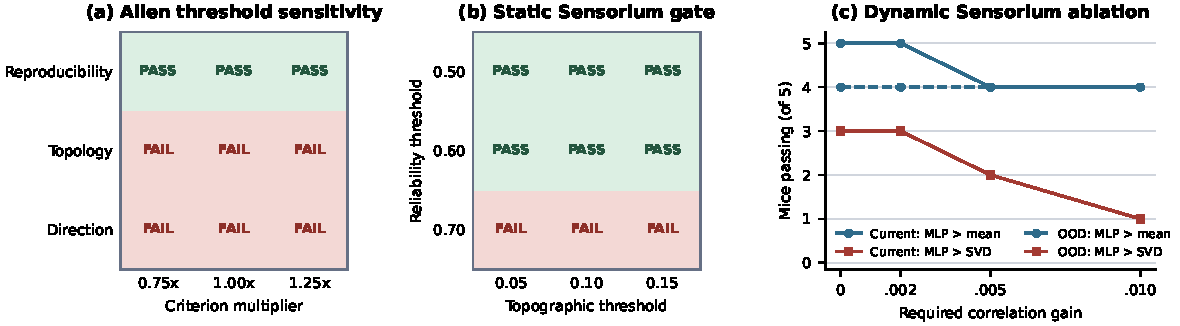
\includegraphics[width=0.88\linewidth]{figures/sensitivity_ablation.pdf}
  \caption{Sensitivity and ablation results for Allen, Static
  Sensorium, and Dynamic Sensorium. Solid lines denote the current cohort and
  dashed lines the legacy out-of-distribution cohort.}
  \label{fig:sensitivity-ablation}
\end{figure}

The Dynamic Sensorium panel provides an ablation over comparator strength and
minimum effect. At zero or 0.002 required gain, the \acs{mlp} exceeds temporal \acs{svd} in
three of five mice in each cohort. At 0.005 this falls to two mice, and at 0.010
to one. By contrast, gains over mean response remain in four or five mice over
the same range. The apparent neural-network advantage is therefore robust to a
weak baseline but not to a stronger temporal decomposition. This result is not
used to reject the \acs{mlp}. It establishes the narrower conclusion that model
complexity alone is not the source of the predictive evidence and that claims
of architectural superiority depend materially on the comparator and minimum
effect selected.

\subsection{RQ3: MICRONS structure--function validation and cross-regime synthesis}
\label{subsec:rq3-microns}

\acs{microns} supplies the local co-registration required for a positive
structure--function test. Data were queried from the public
\path{minnie65_public} \ac{cave} stack. Functional descriptors were obtained from
\path{digital_twin_properties_bcm_coreg_v4}, structural edges were
queried at materialization version 1507, and acquisition artifacts recorded the
datastack, table, materialization, offsets, limits, and source identifiers.
Three non-overlapping ordered windows defined discovery and internal
hold-out reproduction. Offset 0 provided 1000 usable units, offset 1000 provided
992, and offset 2000 provided 999. Structural queries yielded 2267, 2161, and
2147 synapses, corresponding to 2095, 1926, and 1922 unique connected directed
pairs. The windows were evaluated separately rather than pooled before
validation. They are internal windows from the same MICRONS resource and should
not be interpreted as independent-animal replication.

An initial discovery analysis compared connected pairs with random,
distance-matched, and degree-matched non-connected pairs across multiple
functional descriptors. Connected pairs were more similar than random and
degree-matched controls, but the aggregate contrast did not survive distance
matching. Since cortical distance affects both connection probability and
functional organization, this failure blocked the broad positive conclusion.
The diagnostic result was retained and readout-location similarity was selected
as a narrower endpoint before the hold-out windows were evaluated. This sequence
is important: the random control alone would have produced an overstated result,
whereas the distance-matched gate forced a bounded claim that could be
evaluated in predeclared non-overlapping hold-out windows.

For each connected directed pair, random non-connected pairs estimated the
unconditioned contrast, distance-matched pairs controlled for spatial
separation, and degree-matched pairs controlled for unequal participation of
high-degree neurons. The effect $\Delta$ was defined as connected-pair
similarity minus control-pair similarity. One-sided tests evaluated the
declared positive direction, and the Benjamini--Hochberg procedure controlled
the false discovery rate within each stratified family. Because one neuron can
contribute to many pairs, uncertainty was estimated with 300 unit-cluster
bootstrap samples using seed 71. Resampling units induces weights over the existing directed pair frame and
avoids the false precision obtained when derived pairwise observations are
treated as independent.

The three cohorts jointly contained 2991 units, 6575 loaded synapses, and 5943
unique connected directed pairs. Table~\ref{tab:microns-primary} reports the
primary matched effects. The values $\Delta_d$ and $\Delta_k$ denote the
difference between the mean readout-location similarity of connected directed
pairs and the corresponding non-connected null matched by distance or degree.
Positive values indicate that connected pairs are more similar under the
reported functional descriptor. Readout-location similarity is a derived
functional descriptor from the MICrONS digital-twin table and is normalized as
a similarity score for comparison; it is not a direct causal measurement of
synaptic influence. Distance-matched effects were 0.0215, 0.0210, and 0.0179
in discovery, hold-out 1000, and hold-out 2000, with adjusted $q$ values of
0.0076, 0.0070, and 0.0087. Degree-matched effects were 0.0403, 0.0380, and
0.0286, with adjusted $q$ values of 0.0053, 0.0062, and 0.0083. The effect
therefore retained its sign and approximate magnitude outside the window used
to establish the endpoint.

\begin{table}[t]
\centering
\caption{Internally reproduced MICRONS primary endpoint. $\Delta_d$ and $\Delta_k$ are differences between connected-pair readout-location similarity and non-connected nulls matched by distance or degree; positive values indicate greater similarity among connected pairs. The readout-location descriptor is derived and must not be interpreted as causal evidence.}
\label{tab:microns-primary}
\small
\begin{tabular}{lrrrrrr}
\toprule
Cohort & Units & Connected & $\Delta_d$ & $q_d$ & $\Delta_k$ & $q_k$ \\
\midrule
Discovery & 1000 & 2095 & 0.0215 & 0.0076 & 0.0403 & 0.0053 \\
Hold-out 1000 & 992 & 1926 & 0.0210 & 0.0070 & 0.0380 & 0.0062 \\
Hold-out 2000 & 999 & 1922 & 0.0179 & 0.0087 & 0.0286 & 0.0083 \\
\bottomrule
\end{tabular}
\end{table}

Unit-cluster bootstrap stability intervals remained strictly positive in every
cohort (Table~\ref{tab:microns-bootstrap}). Distance-matched lower bounds were
0.0166, 0.0142, and 0.0115. Degree-matched lower bounds were 0.0349, 0.0321,
and 0.0229. All 300 requested bootstrap samples were usable. Because directed
pairs share neurons, these intervals are reported as a unit-cluster stability
analysis and are not treated as if pairwise observations were independent. The
discovery family contained 174 tests across descriptors and strata, of which
28 were confirmed after false-discovery-rate correction. The hold-outs
contained 162 and 174 tests, with 30 and 25 confirmed positives. These counts
describe the multiplicity families and are not presented as independent
biological discoveries. The main claim rests on the fixed readout-location
endpoint and its internal reproduction.

\begin{table}[t]
\centering
\caption{Unit-cluster bootstrap stability analysis for the MICRONS primary endpoint using 300 resamples per cohort. PI denotes a 95\% percentile interval. Intervals are reported as robustness summaries for neuron-sharing pair data, not as naive pair-level uncertainty estimates.}
\label{tab:microns-bootstrap}
\small
\begin{tabular}{lrrrr}
\toprule
Cohort & Distance median & Distance 95\% PI & Degree median & Degree 95\% PI \\
\midrule
Discovery & 0.0218 & [0.0166, 0.0263] & 0.0405 & [0.0349, 0.0454] \\
Hold-out 1000 & 0.0209 & [0.0142, 0.0263] & 0.0377 & [0.0321, 0.0431] \\
Hold-out 2000 & 0.0181 & [0.0115, 0.0238] & 0.0287 & [0.0229, 0.0354] \\
\bottomrule
\end{tabular}
\end{table}

The \acs{microns} outcome is an internally reproduced local observational association, not a new
wiring rule or a causal mechanism. Readout-location similarity may still covary
with cell type, layer, cortical area, morphology, or developmental organization.
Distance and degree matching address two major confounds but do not exhaust the
causal graph. Moreover, Ding et al. reported a substantially richer analysis of
like-to-like connectivity using receptive fields, feature preference, and
axon--dendrite geometry \citep{ding2025wiring}. The present result serves as a
connectomic validation case for the audit: it shows that MouseBrainBench can admit a
positive, internally reproduced claim without asserting priority over the
underlying biological phenomenon.

Table~\ref{tab:cross-regime-results} brings the complete evaluation together.
The important outcome is not that one resource attains the highest score. The
same executable logic represents complete synthetic passage, incomplete
mechanistic systems, reproducible but non-identifying Allen activity,
predictive Sensorium models, and a local positive \acs{microns} association without
semantic promotion. Compared with a conventional evaluation that mainly reports
prediction or reproducibility, this non-compensatory gate prevents Allen and
Sensorium results from being promoted to mechanistic conclusions and restricts
MICRONS to an internal local association. The publication freeze consequently admits those bounded
interpretations while blocking a complete mouse-brain digital twin,
state-of-the-art Sensorium prediction, causal identifiability, behavioural
claims, and whole-brain extrapolation.

\begin{table*}[t]
\centering
\caption{Cross-regime outcomes produced by the same claim-aware audit. Positive
evidence is retained without promoting it to a stronger interpretation.}
\label{tab:cross-regime-results}
\scriptsize
\begin{tabularx}{\textwidth}{@{}p{2.4cm}p{3.3cm}p{3.3cm}X@{}}
\toprule
Case & Positive evidence & Failed or unavailable evidence & Admissible interpretation \\
\midrule
Synthetic directed truth & All reproducibility, topology, and direction blocks pass with $M=1.000$ & None under the designed mechanism & Complete recovery of the synthetic mechanism \\
Synthetic incomplete cases & Strong partial scores ($M=0.333$--$0.719$) & At least one required topology or direction block fails & Diagnostic partial evidence with mechanistic passage rejected \\
Allen VBN & Cross-mouse correlation 0.891 and split-half correlation 0.990 & Topology block 0.073, failed direction criteria, and complete MIS 0.358 & Reproducible population target without identified organization \\
Static Sensorium & Median best correlation 0.328, repeated-test reliability 0.642, and topographic association 0.177 & Reliability unavailable for non-repeated tiers, with no synaptic graph or causal direction & Predictive utility with partial reliability and topographic evidence \\
Dynamic Sensorium & Best mouse-level correlations 0.427--0.526 and MLP median gain 0.043 over mean response & Small gain over temporal SVD (0.0039), while the bounded official run is not competitive & Temporal predictive evidence and verified software integration \\
MICRONS & Distance-matched effects 0.0215, 0.0210, 0.0179 and positive clustered stability intervals in all cohorts & No intervention, same animal/resource, with residual cell-type, layer, area, and morphology confounding & Internally reproduced local observational structure--function association \\
\bottomrule
\end{tabularx}
\end{table*}
